\subsubsection*{9.}
Pour afficher les contraintes creer par DBAIOT on va utiliser la table USER\_CONSTRAINTS , et
afficher les noms des contraintes(constraint\_name) , type (constraint\_name) , les tables associe (table\_name)

\lstinputlisting[style=sqlstyle]{SQL/Partie5/const.sql}

\begin{center}
    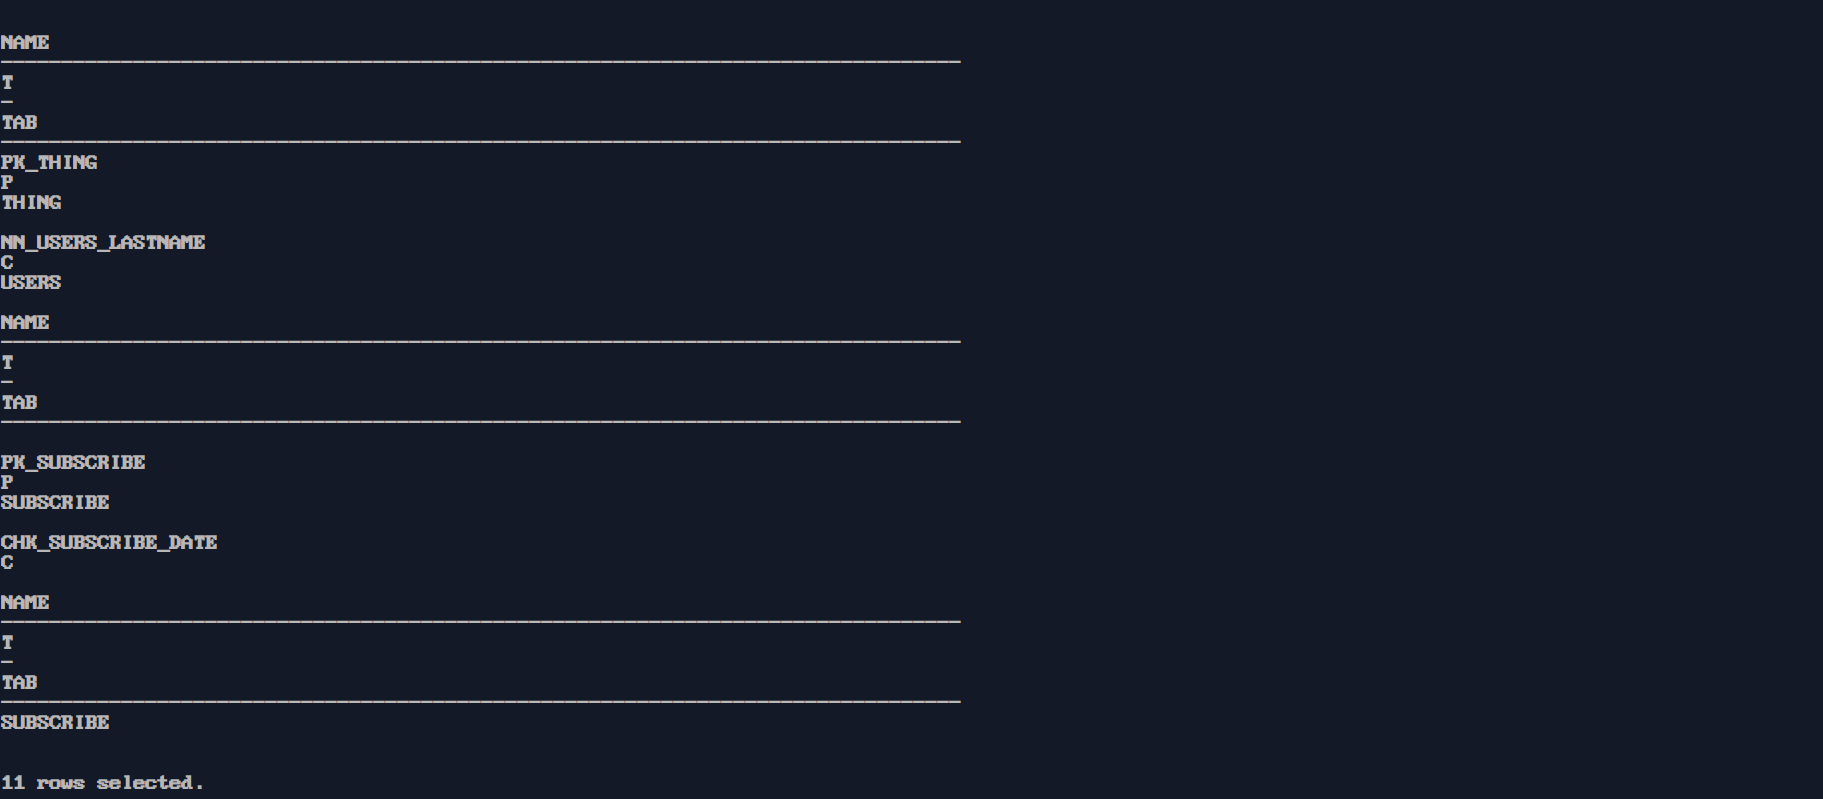
\includegraphics[width=\textwidth]{ScreenShot/Partie5/const.png}
\end{center}


